\documentclass[a4paper]{article}

\usepackage{inputenc}
\usepackage[british,UKenglish]{babel}
\usepackage{amsmath}
%\usepackage{titlesec}
\usepackage{color}
\usepackage{graphicx}
\usepackage{fancyref}
\usepackage{hyperref}
\usepackage{float}
\usepackage{scrextend}
\usepackage{setspace}
\usepackage{xargs}
\usepackage{multicol}
\usepackage{nameref}

\usepackage{sectsty}
\usepackage{multicol}
\usepackage{multirow}
\usepackage[procnames]{listings}
\usepackage{appendix}

\newcommand\tab[1][1cm]{\hspace*{#1}}
\hypersetup{colorlinks=true, linkcolor=black}
\interfootnotelinepenalty=10000

\newcommand{\cleancode}[1]{\begin{addmargin}[3em]{3em}\texttt{\textcolor{cleanOrange}{#1}}\end{addmargin}}
\newcommand{\cleanstyle}[1]{\text{\textcolor{cleanOrange}{\texttt{#1}}}}


\usepackage[colorinlistoftodos,prependcaption,textsize=footnotesize]{todonotes}
\newcommandx{\commred}[2][1=]{\textcolor{Red}
{\todo[linecolor=red,backgroundcolor=red!25,bordercolor=red,#1]{#2}}}
\newcommandx{\commblue}[2][1=]{\textcolor{Blue}
{\todo[linecolor=blue,backgroundcolor=blue!25,bordercolor=blue,#1]{#2}}}
\newcommandx{\commgreen}[2][1=]{\textcolor{OliveGreen}{\todo[linecolor=OliveGreen,backgroundcolor=OliveGreen!25,bordercolor=OliveGreen,#1]{#2}}}
\newcommandx{\commpurp}[2][1=]{\textcolor{Plum}{\todo[linecolor=Plum,backgroundcolor=Plum!25,bordercolor=Plum,#1]{#2}}}

\def\code#1{{\tt #1}}

\def\note#1{\noindent{\bf [Note: #1]}}

\makeatletter
%% The "\@seccntformat" command is an auxiliary command
%% (see pp. 26f. of 'The LaTeX Companion,' 2nd. ed.)
\def\@seccntformat#1{\@ifundefined{#1@cntformat}%
   {\csname the#1\endcsname\quad}  % default
   {\csname #1@cntformat\endcsname}% enable individual control
}
\let\oldappendix\appendix %% save current definition of \appendix
\renewcommand\appendix{%
    \oldappendix
    \newcommand{\section@cntformat}{\appendixname~\thesection\quad}
}
\makeatother


% "define" Scala
\usepackage[T1]{fontenc}  
\usepackage[scaled=0.82]{beramono}  
\usepackage{microtype} 

\sbox0{\small\ttfamily A}
\edef\mybasewidth{\the\wd0 }

\lstdefinelanguage{scala}{
  morekeywords={abstract,case,catch,class,def,%
    do,else,extends,false,final,finally,%
    for,if,implicit,import,match,mixin,%
    new,null,object,override,package,%
    private,protected,requires,return,sealed,%
    super,this,throw,trait,true,try,%
    type,val,var,while,with,yield},
  sensitive=true,
  morecomment=[l]{//},
  morecomment=[n]{/*}{*/},
  morestring=[b]",
  morestring=[b]',
  morestring=[b]"""
}

\usepackage{color}
\definecolor{dkgreen}{rgb}{0,0.6,0}
\definecolor{gray}{rgb}{0.5,0.5,0.5}
\definecolor{mauve}{rgb}{0.58,0,0.82}

% Default settings for code listings
\lstset{frame=tb,
  language=scala,
  aboveskip=3mm,
  belowskip=3mm,
  showstringspaces=false,
  columns=fixed, % basewidth=\mybasewidth,
  basicstyle={\small\ttfamily},
  numbers=none,
  numberstyle=\footnotesize\color{gray},
  % identifierstyle=\color{red},
  keywordstyle=\color{blue},
  commentstyle=\color{dkgreen},
  stringstyle=\color{mauve},
  frame=single,
  breaklines=true,
  breakatwhitespace=true,
  procnamekeys={def, val, var, class, trait, object, extends},
  procnamestyle=\ttfamily\color{red},
  tabsize=2
}

\lstnewenvironment{scala}[1][]
{\lstset{language=scala,#1}}
{}
\lstnewenvironment{cpp}[1][]
{\lstset{language=C++,#1}}
{}
\lstnewenvironment{bash}[1][]
{\lstset{language=bash,#1}}
{}
\lstnewenvironment{verilog}[1][]
{\lstset{language=verilog,#1}}
{}



\lstset{frame=,basicstyle={\footnotesize\ttfamily}}

\graphicspath{ {images/} }
\usepackage{ctex}
\usepackage{verbatim}
\usepackage{enumerate}
\usepackage{geometry}
\usepackage{amssymb}
\usepackage{amsmath}
%\usepackage{slashbox}
\usepackage{diagbox}
\usepackage{pifont}%\ding{192} \ding{172}
\usepackage{tikz}
\usepackage{booktabs}
\usepackage{float}
\usepackage{bm}
%\geometry{a4paper, scale=0.72}
\geometry{a4paper,left=2.5cm,right=2.5cm,top=2.5cm,bottom=2.5cm}
%%%%%%%%%%%%%%%%%%%%%%%%%%%%%%%%%%%%%%%% BEGIN DOC %%%%%%%%%%%%%%%%%%%%%%%%%%%%%%%%%%%%%%%%

\begin{document}
\setlength{\abovecaptionskip}{0pt}
\setlength{\belowcaptionskip}{0pt}
\renewcommand{\contentsname}{目\ 录}
\renewcommand{\appendixname}{附录}
\renewcommand{\appendixpagename}{附录}
\renewcommand{\refname}{参考文献} 
\renewcommand{\figurename}{图}
\renewcommand{\tablename}{表}
\renewcommand{\today}{\number\year 年 \number\month 月 \number\day 日}
\renewcommand{\comma}{$\mkern -8.5mu\raise -.2ex\hbox{\rotatebox[]{180}{\`}}\ $}

\newcommand*{\circled}[1]{\lower.7ex\hbox{\tikz\draw (0pt, 0pt)%
    circle (.5em) node {\makebox[1em][c]{\small #1}};}}
\title{{\Huge 近代物理实验报告{\large\linebreak\\}}{\Large 实验1-3:\ X射线标识谱与吸收\linebreak\linebreak}}
%please write your name, Student #, and Class # in Authors, student ID, and class # respectively
\author{\\姓\ 名:付\ 大\ 为\\
学\ 号: 1800011105\\
邮\ 箱: \url{fudw@pku.edu.cn}\\
%班\ 号: xxxxx\\\\
近代物理实验 (I)\\
(2021,秋季学期)\\\\
北京大学\\
物理学院\\
2018级1班}
\date{\today}
\maketitle
\newpage

%%%%%%%%%%%%%%%%%%%%%%%%%%%%%%%%%%%%%%%% ABSTRACT %%%%%%%%%%%%%%%%%%%%%%%%%%%%%%%%%%%%%%%%
\begin{center}
{\Large\bf{摘\ 要\\}}
\end{center}

当原子的外层电子向内壳层上的空位跃迁时,会放出X射线光子.对于不同的原子,因为其电子壳层结构的不同,其放出的X射线光子的频率谱是不同的.这一频率谱可以用来唯一地标识和测量某一种特定的元素,被称为X射线的标识谱.在今天X射线标识谱技术已经被广泛地用于各个领域的技术之中.本实验通过验证性实验,证明了X射线标识谱和对应谱的原子的原子序数之间的关系-莫塞莱定律,并且对于X射线与物质的相互作用引发的吸收效应做了研究.\\\\
{\bf{关键词}: }X射线,吸收,标识谱
\newpage

%%%%%%%%%%%%%%%%%%%%%%%%%%%%%%%%%%%%%%%% CONTENT %%%%%%%%%%%%%%%%%%%%%%%%%%%%%%%%%%%%%%%%
\begin{center}
\tableofcontents\label{c}
\end{center}
\newpage

%%%%%%%%%%%%%%%%%%%%%%%%%%%%%%%%%%%%%%%% Introduction %%%%%%%%%%%%%%%%%%%%%%%%%%%%%%%%%%%%%%%%
\section{引言} \label{overview}%------------------------------
1895年德国物理学家伦琴在研究阴极射线时发现了一种新的射线,它不能使用肉眼观察到,但是可以使铂氰化钡的荧光屏发出荧光.当时伦琴将这一新射线称为X射线.后来为了纪念这一射线的发现者,也将它称为伦琴射线.

X射线具有直线传播,经过电场不产生偏转,并且穿透力很强的特征.在其发现后不久,它就被学界用作检查人体伤病的工具,并用来检查金属或者其他物件内部的缺陷.1912年劳厄等人研究了X射线在晶体上的衍射现象,证明了X射线本质上是一种电磁波,波长在\SI{0.1}{nm}左右.1913-1914年莫塞莱发现了元素发出的标识X射线能量与原子序数之间的关系,即莫塞莱定律.
利用莫塞莱定律,1923年人们发现了元素铪.随着闪烁计数器,硅探测器等X射线能谱测量仪器的发展,利用标识X射线来确定材料的化学组成已经广泛地应用于各种现代谱仪分析技术中.

由于X射线的这些优越的特性与广泛的应用,对于X射线的标识谱所满足的物理规律和X射线与物质相互作用所满足的物理规律的研究自然具有实在意义.本实验从这个出发点出发,验证了X射线标识谱所遵守的莫塞莱定律,并且尝试研究了固体对于X射线的吸收过程的相关规律.


%%%%%%%%%%%%%%%%%%%%%%%%%%%%%%%%%%%%%%%% Theory %%%%%%%%%%%%%%%%%%%%%%%%%%%%%%%%%%%%%%%%
\newpage
\section{理论} \label{theory}%------------------------------
%------------------------------------------------------------
\subsection{X射线标识谱}

原子的内壳层上存在一个电子的空位时,处于较外层的电子将跃迁入内层以填充这个空位,从而使得整个原子系统的总能量降低而趋于稳定.根据玻尔的原子理论,外层电子向内层跃迁时,会发生光辐射,其能量为
\begin{equation}
    \label{eq:Eofphoton}
    h\nu = \frac{2\pi^2m_ee^4}{h^2}(Z - \sigma)^2(\frac{1}{n_1^2} -
    \frac{1}{n_2^2})
\end{equation}

显然,不同原子所辐射出来的荧光光子能量与该原子的能级结构有关,实际上,由于不同种类的原子的能级结构差别足够大,一旦知道X射线荧光的光子能量,我们就可以断定它来自于哪一种原子.因此X射线荧光被称为特征X射线,意指为某种原子所持有.

1913-1914年莫塞莱发现,当X射线管中的阳极材料的原子序数$Z$逐渐增加时,相应同一线系的标识X射线的波长逐渐减小,这种波长的变化是单调地逐渐降低,而不像元素的其他性质那样具有周期性.他还发现阳极材料的标识X射线频率的平方根和原子序数$Z$之间存在线性关系,即:
\begin{equation}
    \label{eq:law}
    \sqrt{\nu} = K(Z - \sigma)
\end{equation}

上式称为莫塞莱定律,式中$K$与$\sigma$都是常数,与式~\ref{eq:Eofphoton}相互比较可以得到常数:
\begin{equation}
    K = \left[\frac{2\pi^2me^4}{h^3}\left(\frac{1}{n_1^2} -
            \frac{1}{n_2^2}\right)\right]^{\frac{1}{2}}
\end{equation}

%------------------------------------------------------------
\subsection{X射线的吸收}

一束强度为$I_0$,光子能量单一的X射线垂直入射到吸收介质上,由于和吸收介质中原子的相互作用,出射的X射线强度会衰减.当介质厚度很薄时,入射X射线束的强度的相对减少量与吸收层厚度成正比:
\begin{equation}
    \label{eq:dII}
    \frac{dI}{I} = - \mu_0 dx
\end{equation}

比例常数$\mu_0$称为线衰减系数.

对于X射线来说,线衰减的主要原因是由于线吸收效应(与吸收介质之间发生的光电效应、康普顿散射和正负电子对产生),而不是弹性散射.并且当X光子的能量在几十\si{keV}时,最主要的相互作用是光电效应,于是有
\begin{equation}
    \mu_0 \approx \tau_{\text{absorption}} \approx \tau_e
\end{equation}

在式~\ref{eq:dII}上积分得到
\begin{equation}
    \label{eq:II0}
    I = I_0 \exp( - \tau_e x)
\end{equation}

设$\rho$是吸收介质的密度,则式~\ref{eq:II0}可以改写为
\begin{equation}
    I = I_0\exp[-(\tau_e/\rho)\rho x] = I_0\exp(-\tau_m\rho x)
\end{equation}

式中$\tau_m$称为相应于光电效应的质量吸收系数,实际工作中采用此式更为方便.

考虑到原子散射光子的具体过程,应有关系
\begin{equation}
    \tau_m \propto \frac{Z^4}{A}\lambda^3
\end{equation}
%%%%%%%%%%%%%%%%%%%%%%%%%%%%%%%%%%%%%%%% Experiment %%%%%%%%%%%%%%%%%%%%%%%%%%%%%%%%%%%%%%%%
\newpage
\section{实验} \label{experiment}%------------------------------

\subsection{实验仪器}
\begin{enumerate}[(1)]
    \item 硅漂移探测器
    \item 放射源
    \item 微机多道分析器
    \item 铅块
    \item 光电倍增管
    \item 高压电源
    \item 电脑(内含数据处理软件)
\end{enumerate}

\begin{comment}
\subsection{简要实验步骤}\label{sub:ExperimentalSteps}
\begin{enumerate}[1.]
    \item 连接实验装置.先用脉冲发生器作输入信号源,用示波器观察各级输出,调节放大倍数,使得线性放大器输出的脉冲幅度为5~6V.
    \item 用示波器观察
    \item
    \item
\end{enumerate}

\circled{1}抽真空(按橘色按钮),约2分钟,机械泵声音平稳即可\\\\
\end{comment}
%%%%%%%%%%%%%%%%%%%%%%%%%%%%%%%%%%%%%%%% Results & Discussions %%%%%%%%%%%%%%%%%%%%%%%%%%%%%%%%%%%%%%%%
\newpage
\section{结果及分析}

%------------------------------------------------------------
\subsection{验证莫塞莱定律(必做Mo、Sr、Se、Zn、Ni、Fe)}\label{sub1}
$t=120s$,
测量结果如下\textbf{表~\ref{tab:table1}.}
\begin{table}[H]
\caption{\textbf{不同材料的特征X射线}}
\label{tab:table1}
\begin{center}
\setlength{\tabcolsep}{7mm}
\begin{tabular}{|c|c|c|c|}%p{6cm}|}
    \toprule
	\hline
	材料 & 峰位置 & 半高宽(FWHM) & 计数率 \\ \hline \hline
	Mo & 1757.23 & 25.2990 & $117.94\pm1.04$ \\ \hline
	Sr & 1427.48 & 23.8148 & $360.79\pm1.80$ \\ \hline
	Se & 1132.46 & 21.1784 & $472.13\pm2.03$ \\ \hline
	Zn & 873.61 & 20.1403 & $526.88\pm2.16$ \\ \hline
	Ni & 757.26 & 19.4102 & $278.72\pm1.59$ \\ \hline
	Fe & 649.04 & 18.3430 & $256.77\pm1.51$ \\ \hline
	\bottomrule
	\end{tabular}
\end{center}
\end{table}
我们认为特征谱线的光子能量正比于谱线峰位置,这样可以把光子的频率用相对单位表示,对\textbf{表~\ref{tab:table1}}的数据做直线拟合,得到如\textbf{图~\ref{fig:fig1}}所示结果:
\begin{figure}[H]
 \centering
 \caption{验证莫塞莱定律}
 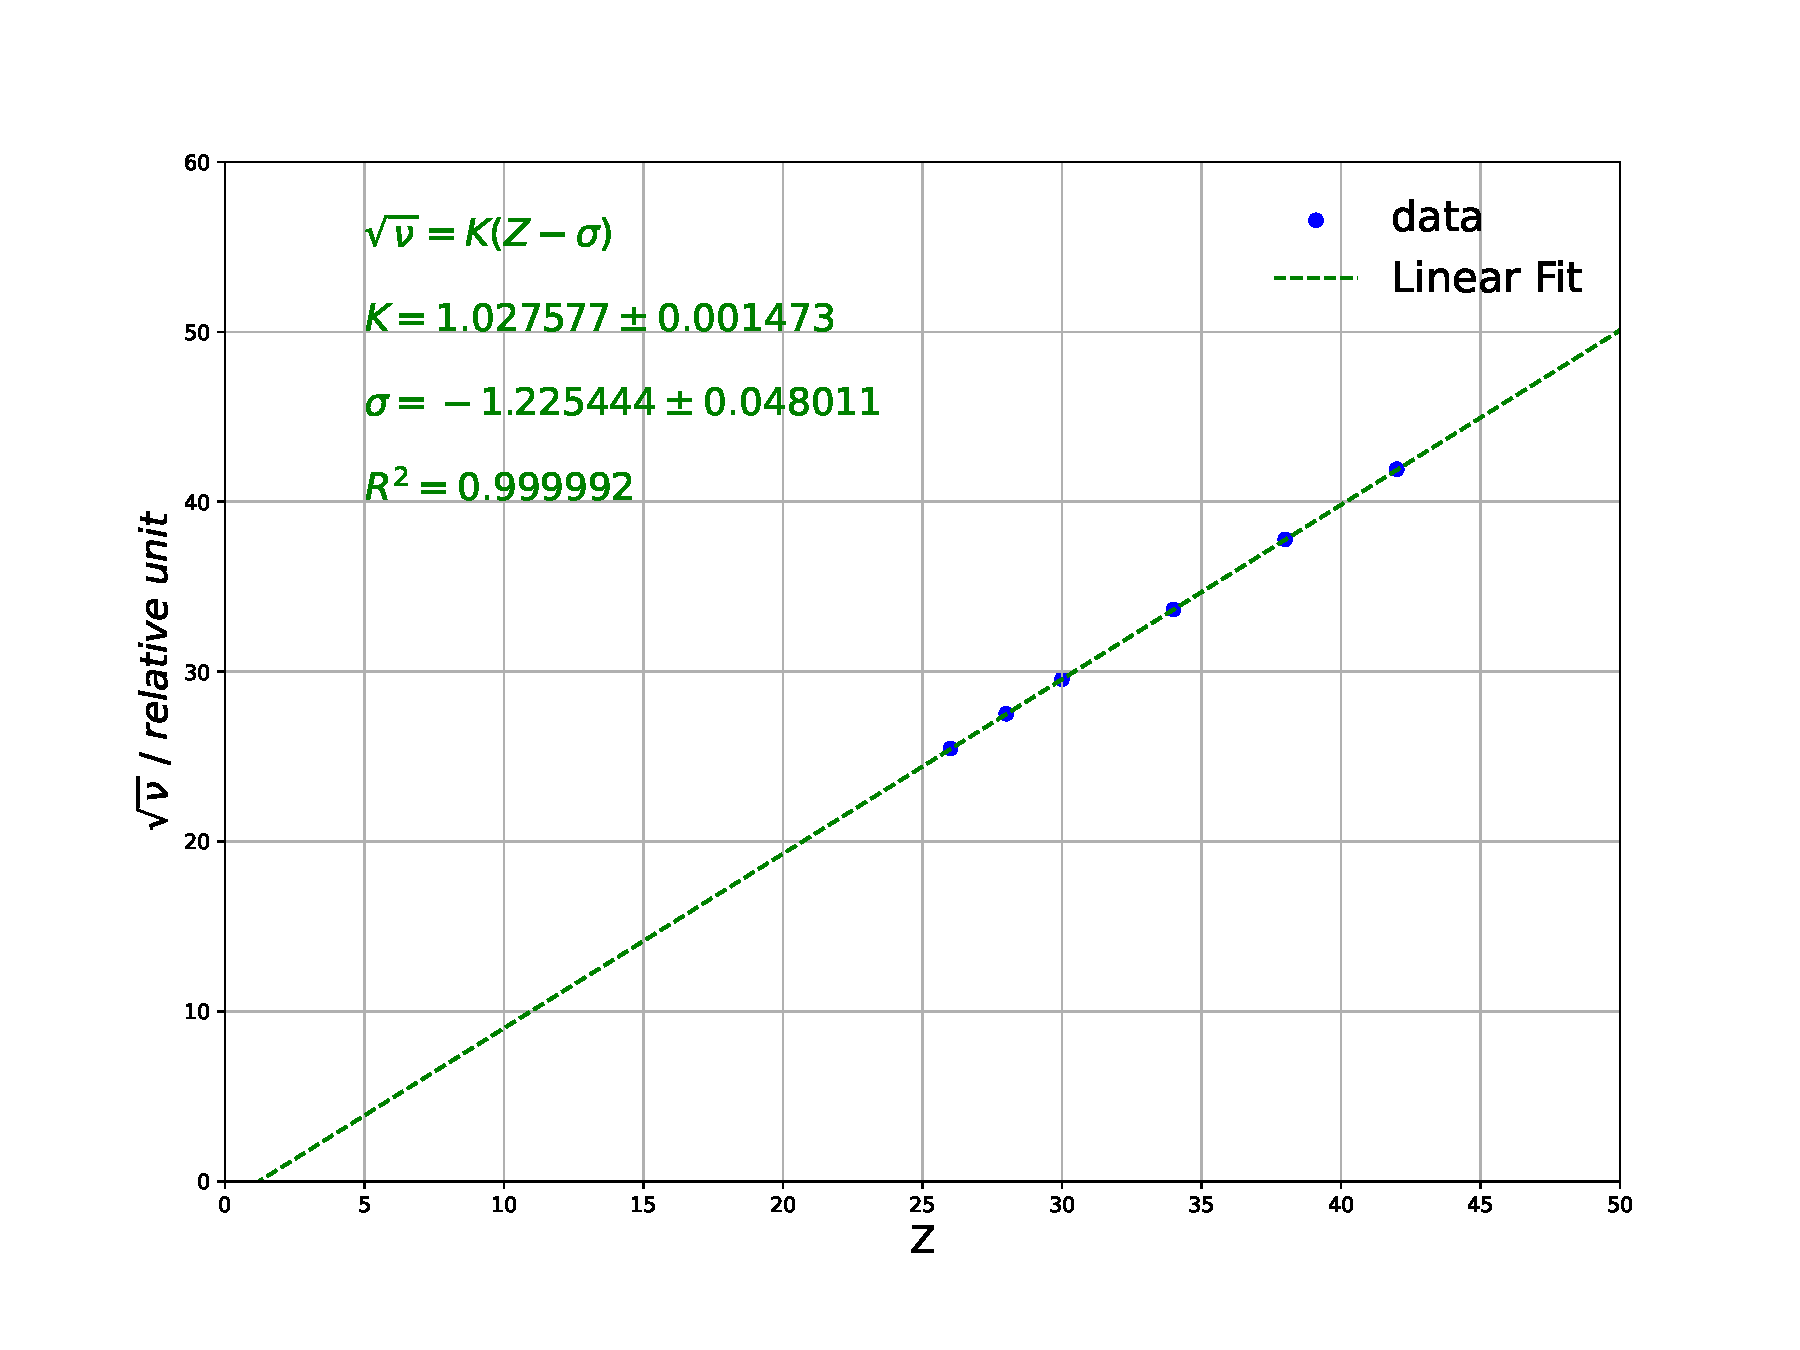
\includegraphics[height=12cm, width=16cm]{images/phyex1_fig.pdf}
 \label{fig:fig1}
\end{figure}
%------------------------------------------------------------
\subsection{吸收实验(获取时间120s即可):Mo、Sr、Se、Zn、Ni、Fe}\label{sub2}
我们首先知道单块Al片的厚度为$d=\sigma_{Al}/\rho_{Al}=1.963\times10^{-3}\rm cm$.

不同厚度铝片对来自Mo的X射线测量结果如下\textbf{图~\ref{fig:fig2}}.
\begin{figure}[H]
 \centering
 \caption{不同厚度铝片对来自Mo的X射线测量结果}
 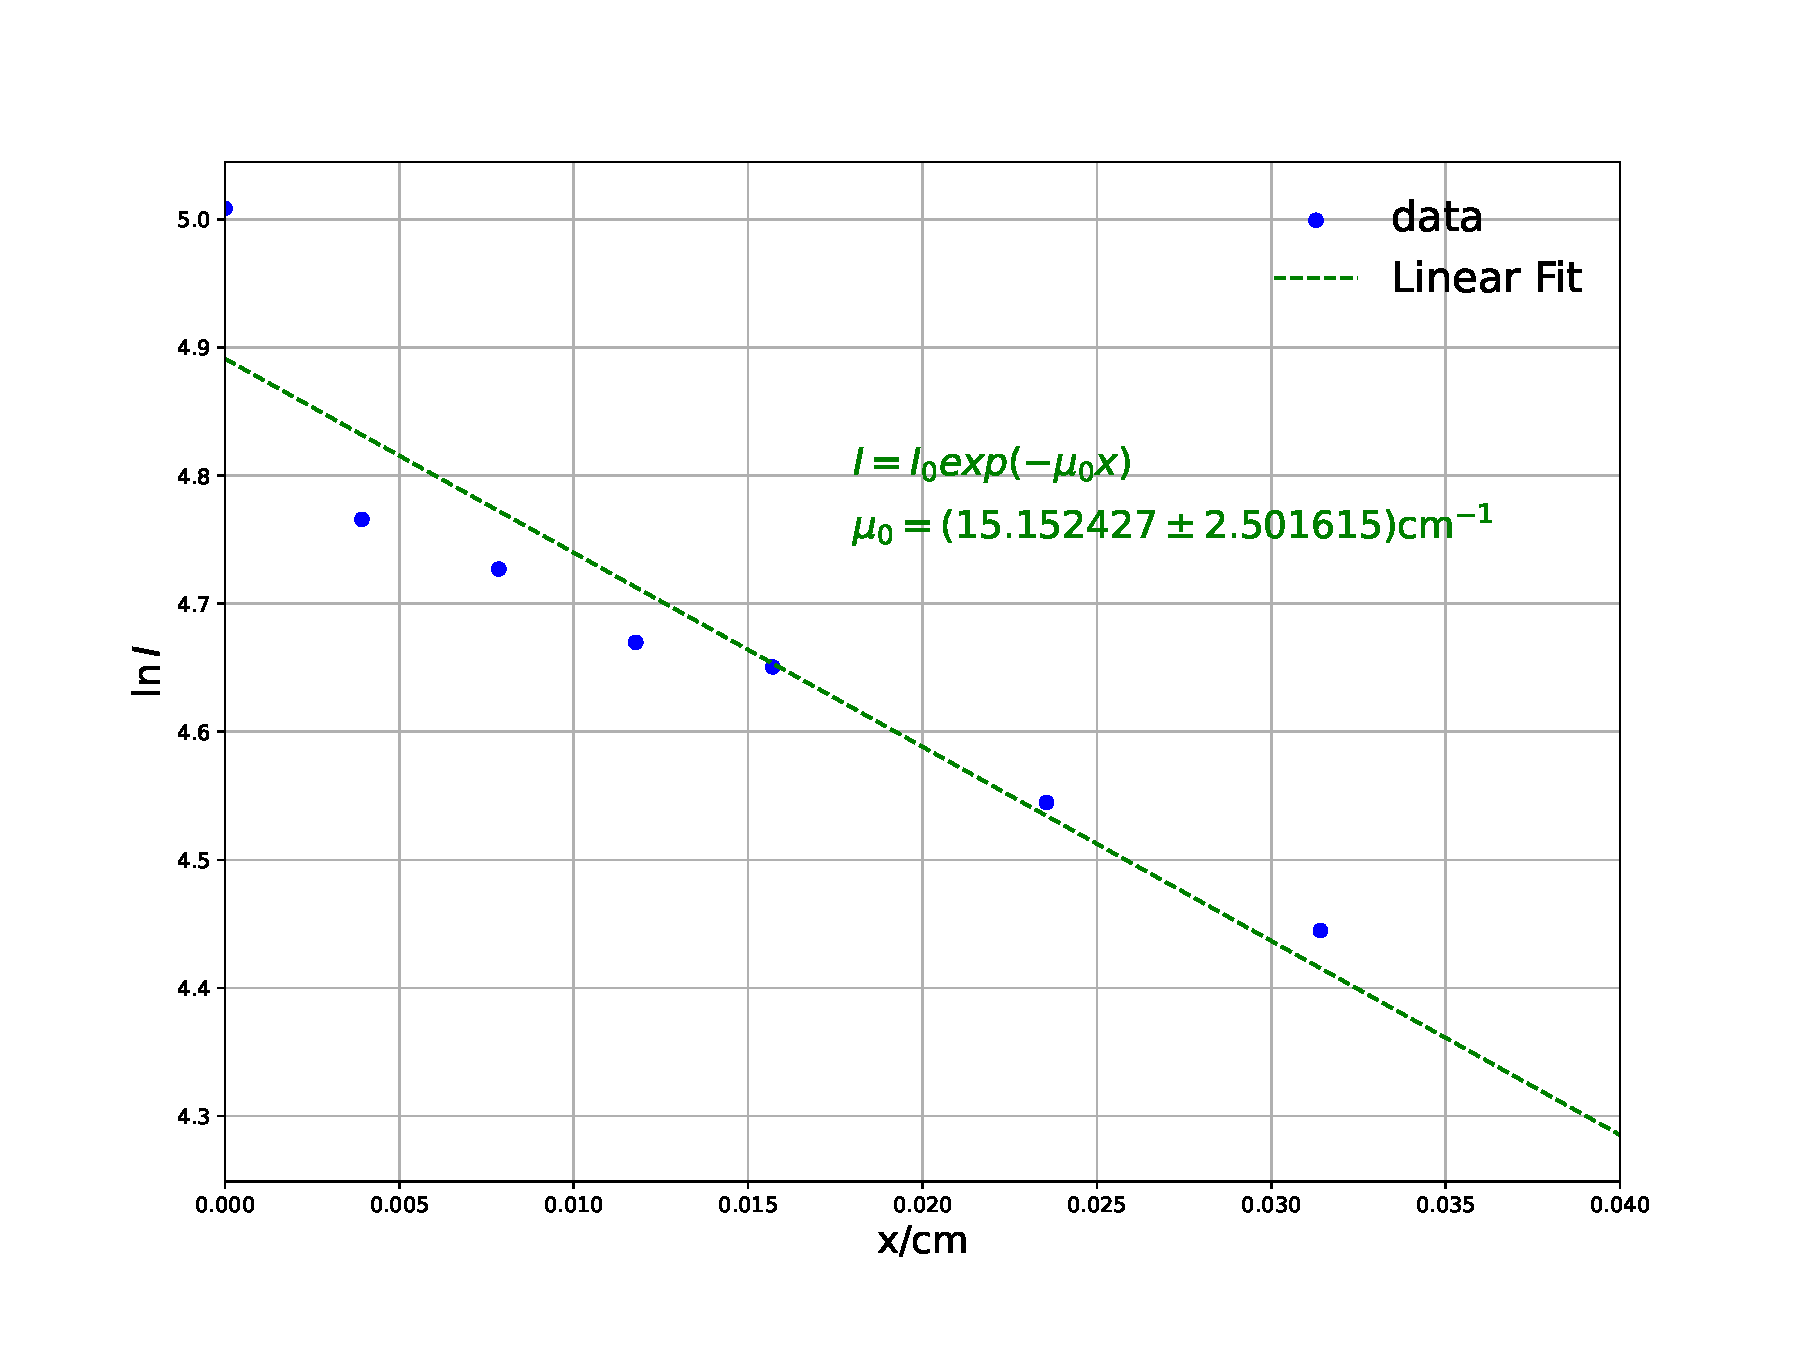
\includegraphics[height=10.5cm, width=14cm]{images/phyex2_fig1.pdf}
 \label{fig:fig2}
\end{figure}
不同厚度铝片对来自Sr的X射线测量结果如下\textbf{图~\ref{fig:fig3}}.
\begin{figure}[H]
 \centering
 \caption{不同厚度铝片对来自Sr的X射线测量结果}
 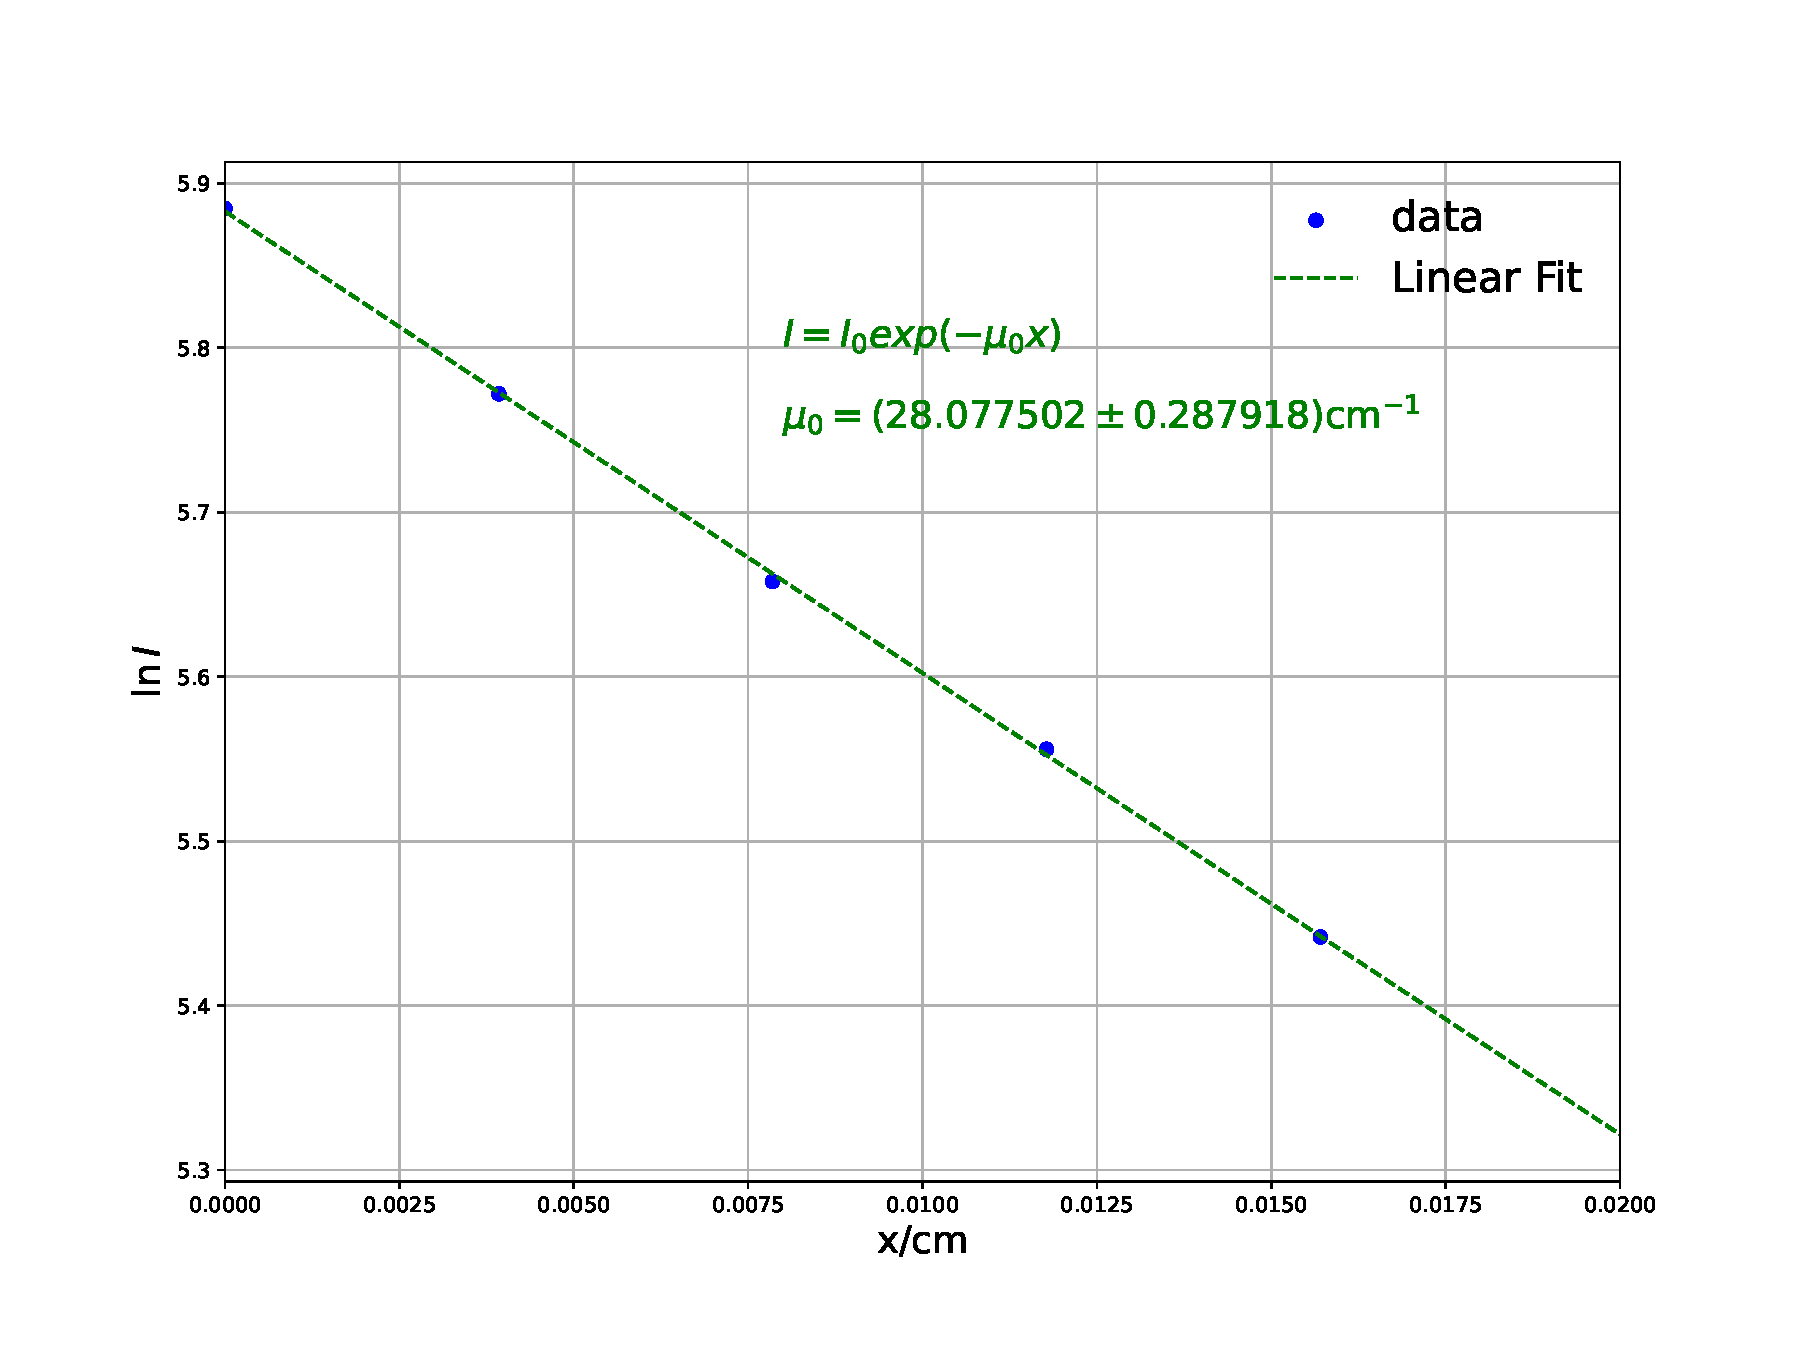
\includegraphics[height=10.5cm, width=14cm]{images/phyex2_fig2.pdf}
 \label{fig:fig3}
\end{figure}
不同厚度铝片对来自Zn的X射线测量结果如下\textbf{图~\ref{fig:fig4}}.
\begin{figure}[H]
 \centering
 \caption{不同厚度铝片对来自Zn的X射线测量结果}
 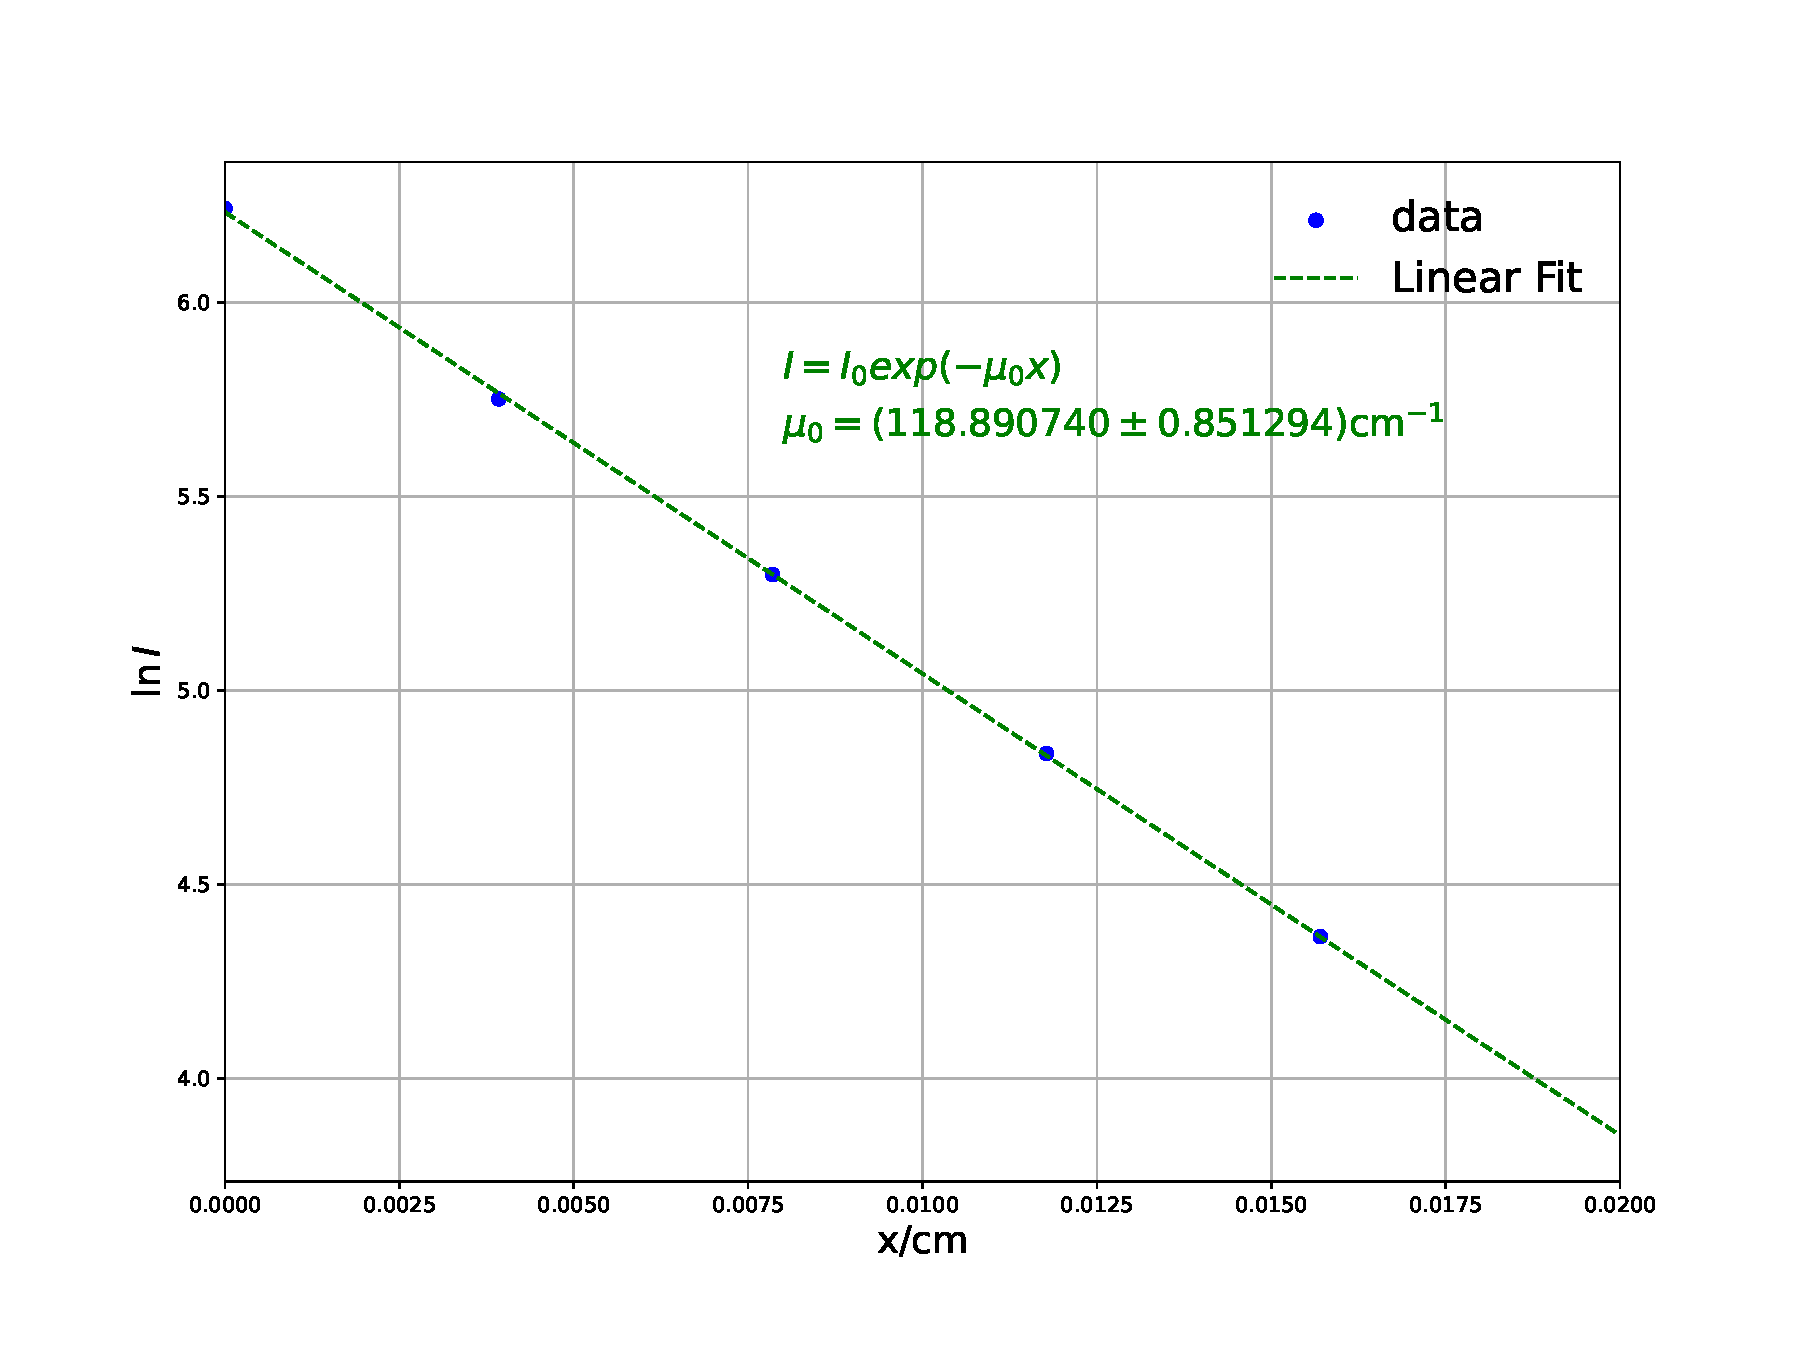
\includegraphics[height=10.5cm, width=14cm]{images/phyex2_fig3.pdf}
 \label{fig:fig4}
\end{figure}
不同厚度铝片对来自Ni的X射线测量结果如下\textbf{图~\ref{fig:fig5}}.
\begin{figure}[H]
 \centering
 \caption{不同厚度铝片对来自Ni的X射线测量结果}
 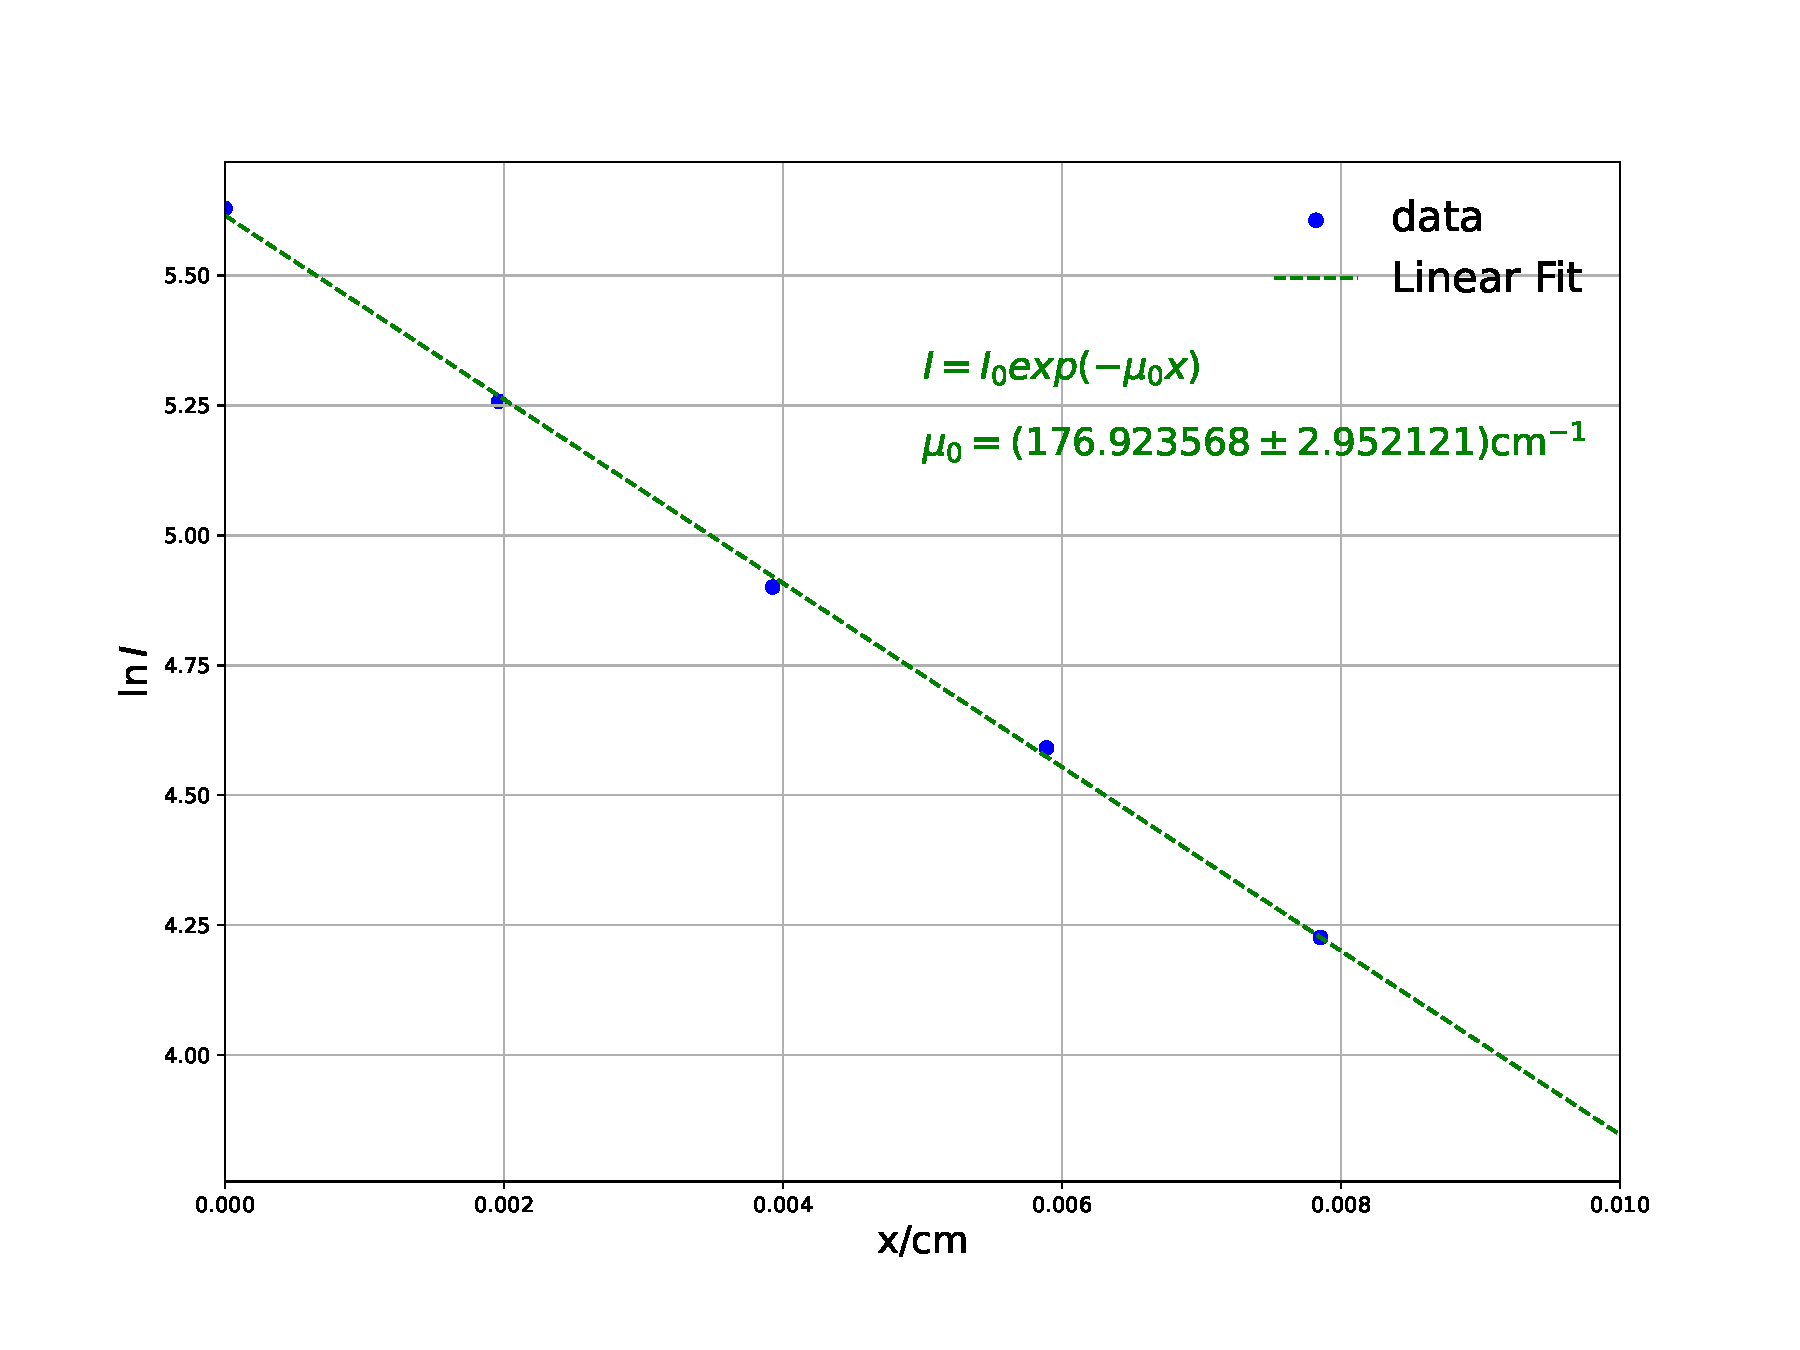
\includegraphics[height=10.5cm, width=14cm]{images/phyex2_fig4.pdf}
 \label{fig:fig5}
\end{figure}
不同厚度铝片对来自Fe的X射线测量结果如下\textbf{图~\ref{fig:fig6}}.
\begin{figure}[H]
 \centering
 \caption{不同厚度铝片对来自Fe的X射线测量结果}
 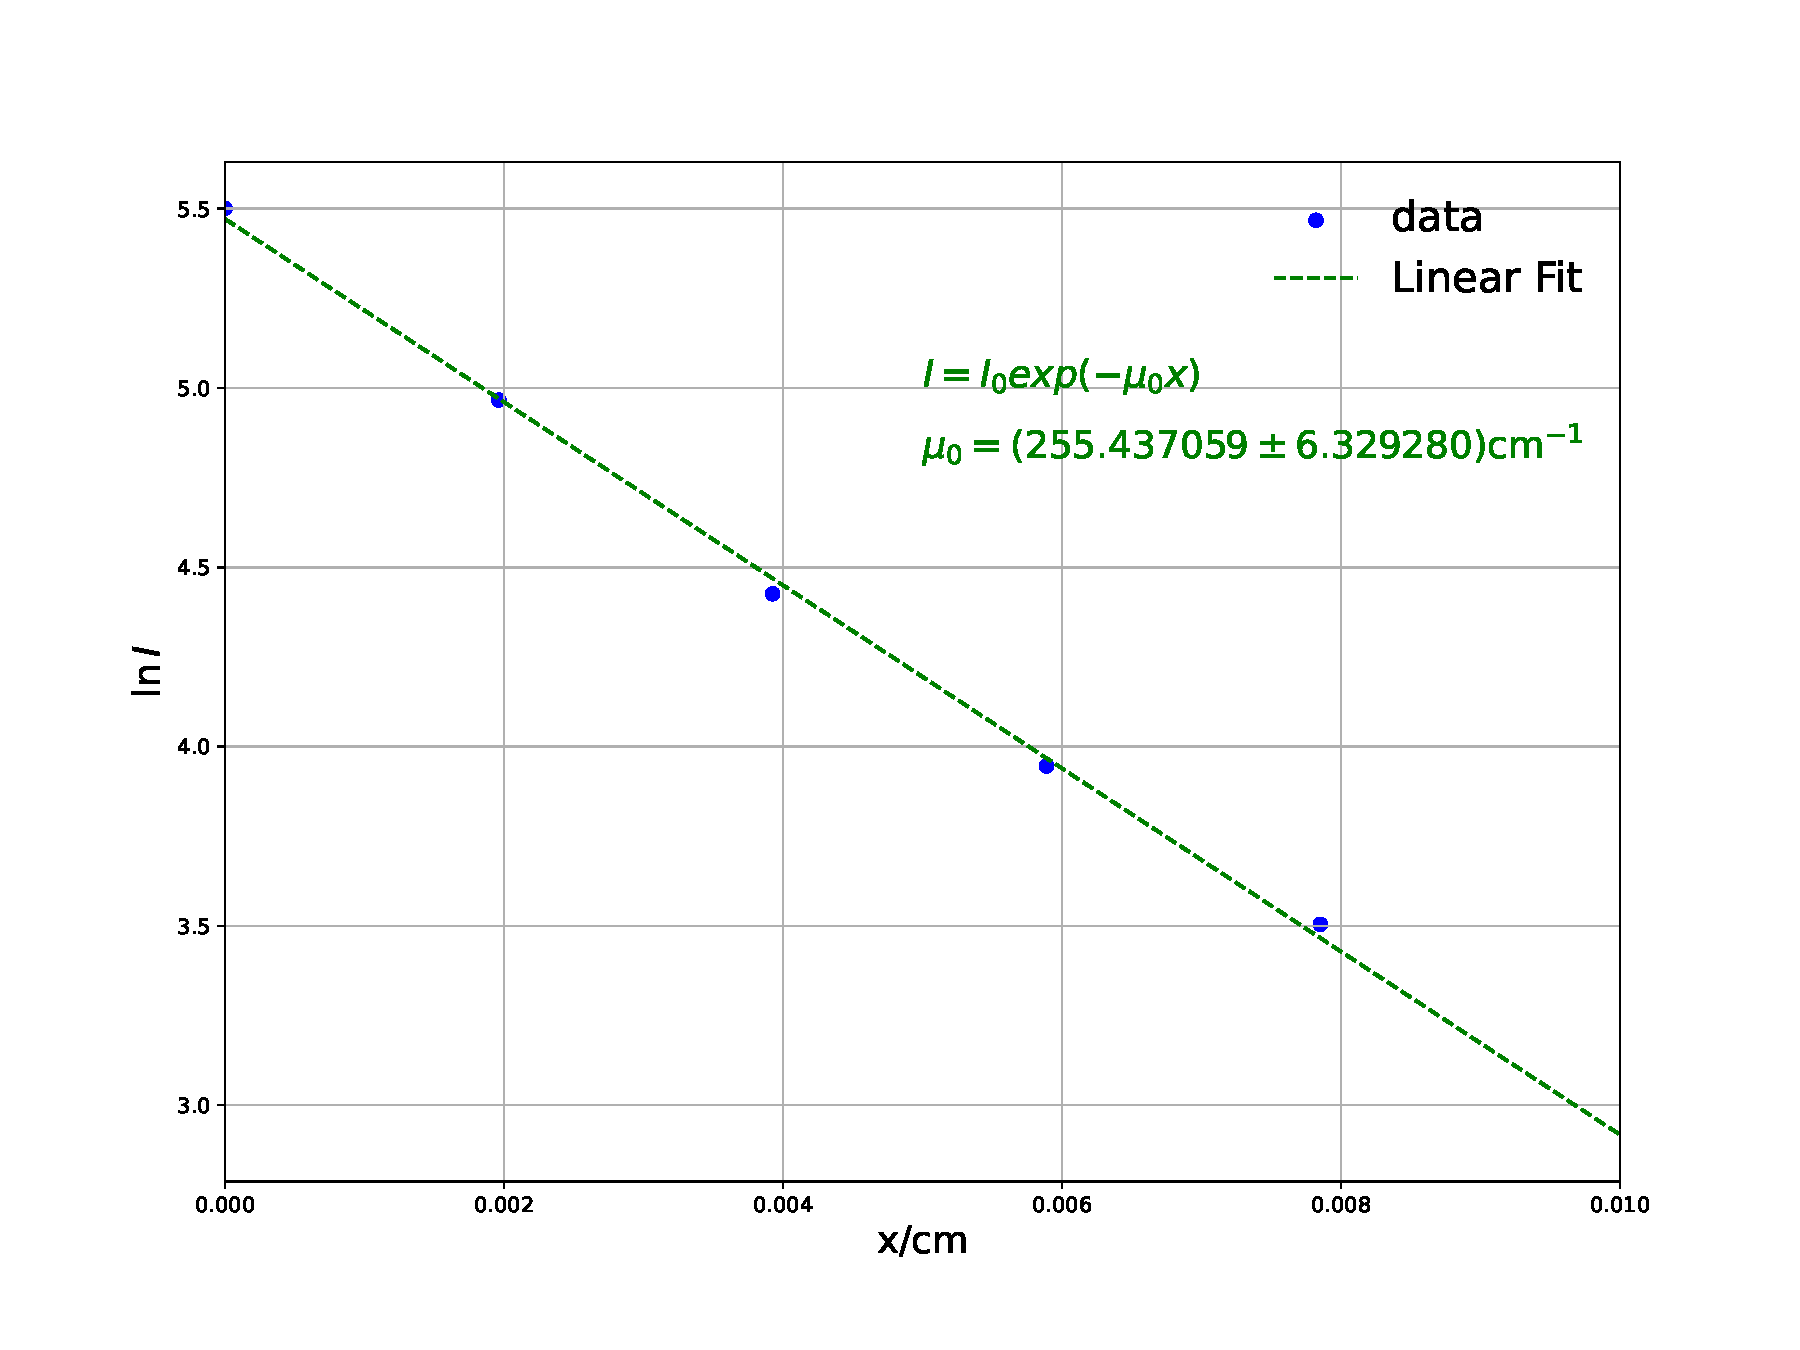
\includegraphics[height=10.5cm, width=14cm]{images/phyex2_fig5.pdf}
 \label{fig:fig6}
\end{figure}
这样得到铝片对不同材料的标识X射线吸收结果汇总如下\textbf{表~\ref{tab:table2}.}
\begin{table}[H]
\caption{\textbf{铝片对不同材料的标识X射线吸收测量}}
\label{tab:table2}
\begin{center}
\setlength{\tabcolsep}{7mm}
\begin{tabular}{|c|c|c|c|}%p{6cm}|}
    \toprule
	\hline
	材料 & 峰位 & $\mu_0=\tau_e/\rm cm^{-1}$ & $\tau_m=\frac{\tau_e}{\rho}/\rm (cm^2/g)$ \\ \hline \hline
	Mo & 1757.23 & 15.15 & 5.61 \\ \hline
	Sr & 1427.48 & 28.08 & 10.40 \\ \hline
	Zn & 873.61 & 118.89 & 44.03 \\ \hline
	Ni & 757.26 & 176.92 & 65.53 \\ \hline
	Fe & 649.04 & 255.44 & 94.61 \\ \hline
	\bottomrule
	\end{tabular}
\end{center}
\end{table}

我们这里仍然用峰位近似代替光子频率$\nu$,并且有$\lambda=c/\nu$,从而可以验证$\tau_m\propto\frac{Z^4}{A}\lambda^3$关系,如下\textbf{图~\ref{fig:fig7}}所示结果:
\begin{figure}[H]
 \centering
 \caption{验证$\tau_m\propto\frac{Z^4}{A}\lambda^3$}
 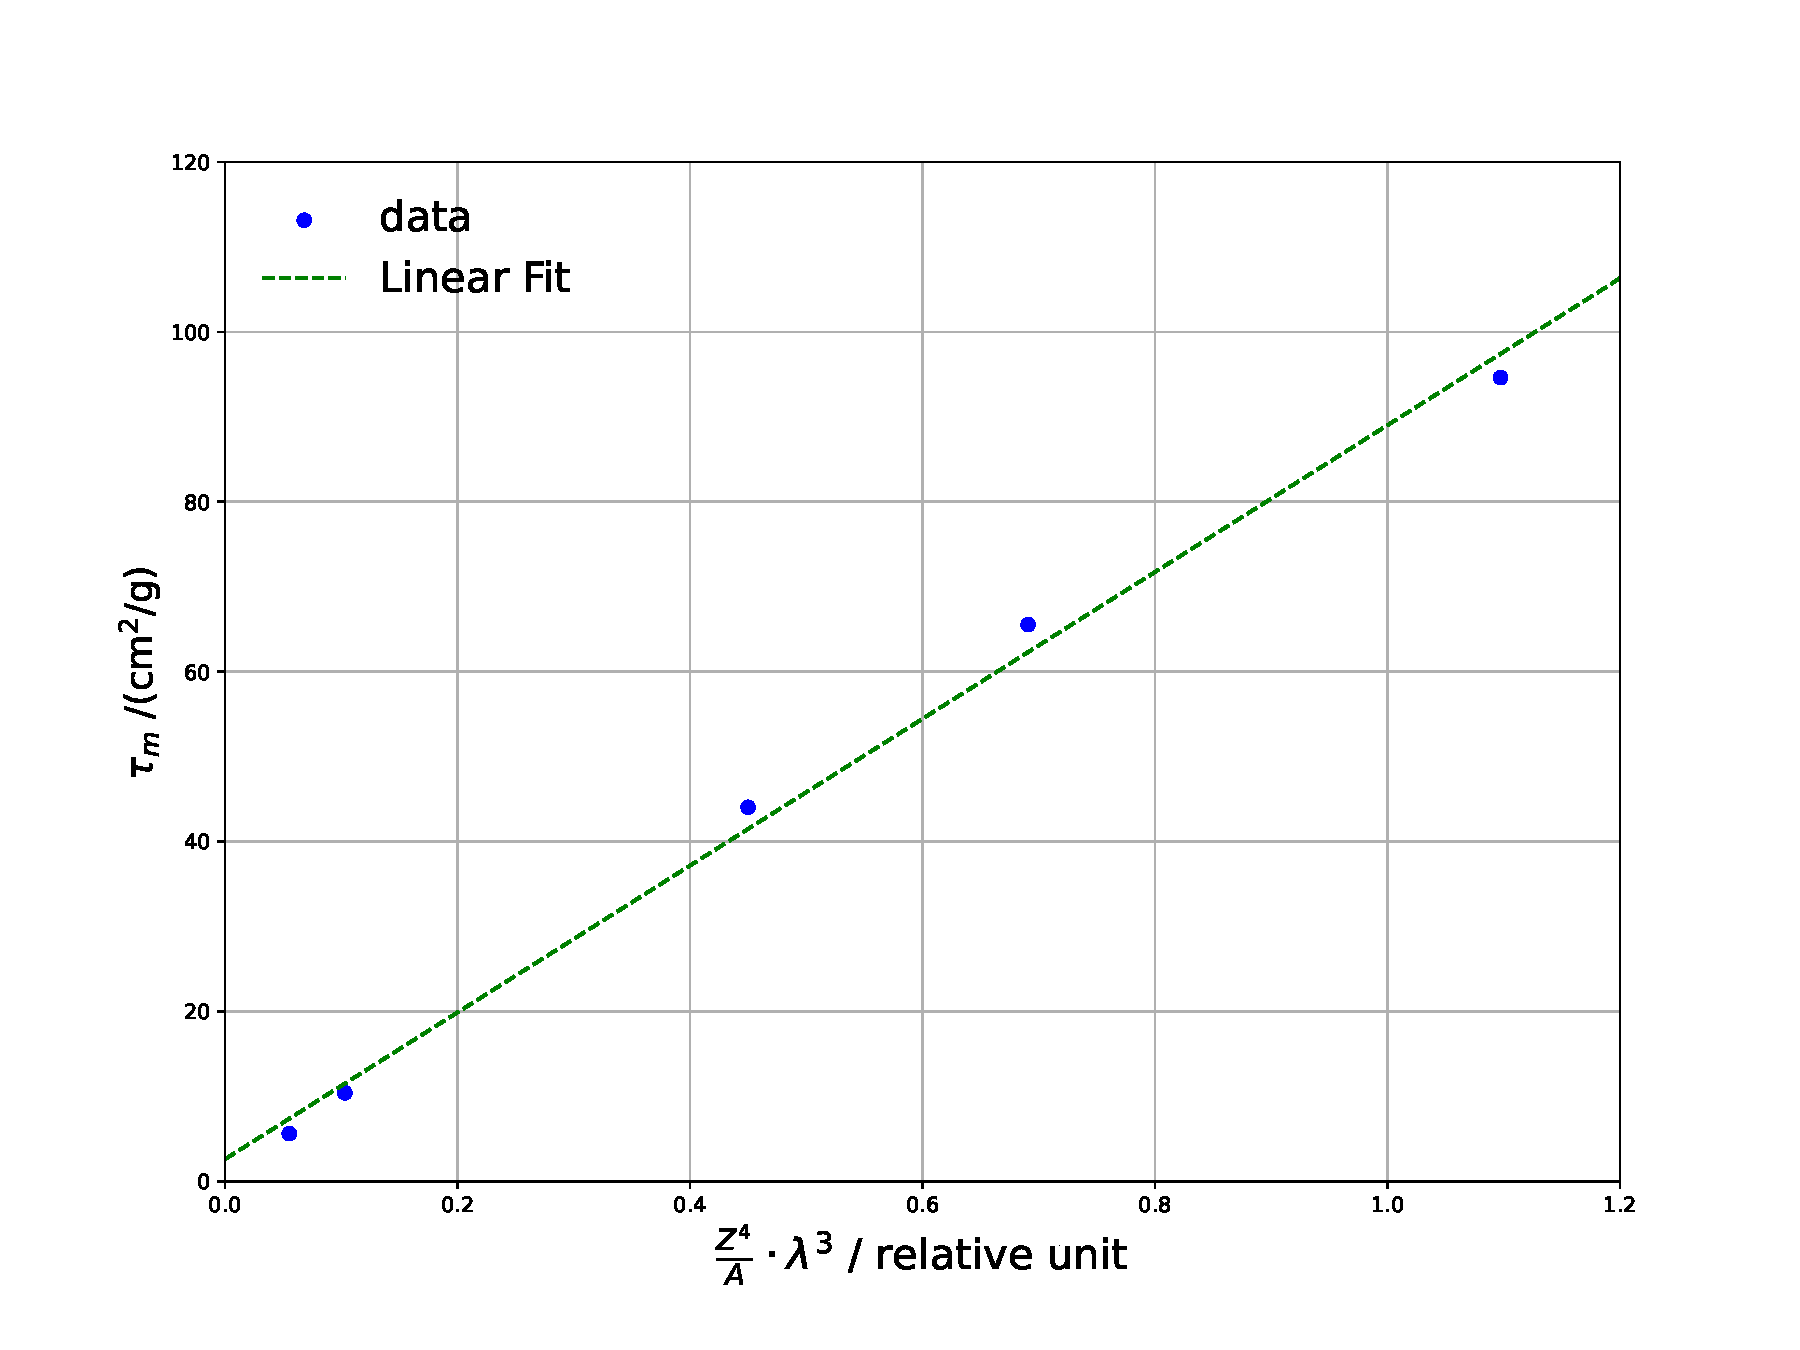
\includegraphics[height=12cm, width=16cm]{images/phyex2_fig6.pdf}
 \label{fig:fig7}
\end{figure}
通过实验结果验证了$\tau_m$和$\lambda$的理论关系
%%%%%%%%%%%%%%%%%%%%%%%%%%%%%%%%%%%%%%%% Conclusion %%%%%%%%%%%%%%%%%%%%%%%%%%%%%%%%%%%%%%%%
\newpage
\section{结论}\label{conclusions}
本实验成功地验证了莫塞莱定律所指出的原子的标识X射线频率的平方根和原子序数之间的线性关系,并且对于X射线在吸收介质中的吸收规律作出有意义的实验测量和验证.\\
\begin{comment}
%%%%%%%%%%%%%%%%%%%%%%%%%%%%%%%%%%%%%%%% Questions %%%%%%%%%%%%%%%%%%%%%%%%%%%%%%%%%%%%%%%%
\section{实验报告思考题}\label{questions}
\subsection{分析本实验的主要误差来源,试述有限立体角的影响和减少实验误差的办法}\label{sub:question1}
答:减少实验误差:本实验中仅取3点标定了系统的能量刻度,相
应的线性拟合结果虽具有充分大的相关性系数,但其误差显著,不可忽略;后续可采
用更丰富的峰值数据进行定标,以提升能量刻度的准确性.
\subsection{讨论实验值与理论值不完全符合的原因}\label{sub:question2}
答:据图线和数据可知,实测能量较理论值普遍有偏差,但偏差不甚显著;而相对截面
的偏差则比较显著.简要分析可知,上述偏差应当主要源于实验
环境的非理想性;事实上,本实验中有诸多误差来源未能充分控制:\\
a.首先,能量刻度可能不够精准,而关于怎么减少能量刻度误差的办法,可以参考上一问.\\
b.此外,仪器附近物质中的电子均可参与散射过程,而本实验所在的室内环境不甚空旷,势必对散射能谱造成影响.这一影响并不能通过去除本底而完全消除;事实上,加上铝棒后,散射导致光子的角分布比未加铝棒时显著增大,从而四壁对光子的散射效应增强、角分布更广,导致了额外的散射截面.
\\

\end{comment}
%%%%%%%%%%%%%%%%%%%%%%%%%%%%%%%%%%%%%%%% Acknowledgements %%%%%%%%%%%%%%%%%%%%%%%%%%%%%%%%%%%%%%%%

\section{致谢}\label{acknowledgments}
感谢王思广老师在实验中的的悉心指导.

%%%%%%%%%%%%%%%%%%%%%%%%%%%%%%%%%%%%%%%% Cite %%%%%%%%%%%%%%%%%%%%%%%%%%%%%%%%%%%%%%%%
\begin{comment}
如果需要索引参考文献,请使用\cite{Erdos01}, 同时已经将参考文献的项目模版在文末写出。
\end{comment}

\begin{comment}
%%%%%%%%%%%%%%%%%%%%%%%%%%%%%%%%%%%%%%%% Appendix %%%%%%%%%%%%%%%%%%%%%%%%%%%%%%%%%%%%%%%%
\appendix
\section{代码}\label{sub:app.code}
请在附录\ref{sub:app.code}中添加代码。请使用如下Scala的语法高亮描述方法。
\begin{scala}
class TopIO extends Bundle() {
	val boot = Input(Bool()) 
// imem and dmem interface for Tests
	val test_im_wr		= Input(Bool())
	val test_im_rd 		= Input(Bool())
	val test_im_addr 	= Input(UInt(32.W))
	val test_im_in 		= Input(UInt(32.W))
	val test_im_out 	= Output(UInt(32.W))

	val test_dm_wr		= Input(Bool())
	val test_dm_rd 		= Input(Bool())
	val test_dm_addr 	= Input(UInt(32.W))
	val test_dm_in 		= Input(UInt(32.W))
	val test_dm_out 	= Output(UInt(32.W))

	val valid			= Output(Bool())
}
class Top extends Module() {
	val io 		= IO(new TopIO())//in chisel3, io must be wrapped in IO(...) 
	//...
	when (io.boot & io.test_im_wr){
		imm(io.test_im_addr) := io.test_im_in
		} .elsewhen (io.boot & io.test_dm_wr){
		// please finish it
		} //...
}
\end{scala}
\newpage

%%%%%%%%%%%%%%%%%%%%%%%%%%%%%%%%%%%%%%%% REFERENCE %%%%%%%%%%%%%%%%%%%%%%%%%%%%%%%%%%%%%%%%
\begin{thebibliography}{9}

\bibitem{Erdos01} P. Erd\H os, \emph{A selection of problems and
results in combinatorics}, Recent trends in combinatorics (Matrahaza,
1995), Cambridge Univ. Press, Cambridge, 2001, pp. 1--6.

\end{thebibliography}
\end{comment}
\end{document}

